% !TEX TS-program = XeLaTeX
% use the following command:
% all document files must be coded in UTF-8
\documentclass[spanish]{textolivre}
% build HTML with: make4ht -e build.lua -c textolivre.cfg -x -u article "fn-in,svg,pic-align"

\journalname{Texto Livre}
\thevolume{15}
%\thenumber{1} % old template
\theyear{2022}
\receiveddate{\DTMdisplaydate{2022}{3}{7}{-1}} % YYYY MM DD
\accepteddate{\DTMdisplaydate{2022}{5}{12}{-1}}
\publisheddate{\DTMdisplaydate{2022}{7}{1}{-1}}
\corrauthor{Francisco Recio-Muñoz}
\articledoi{10.35699/1983-3652.2022.38649}
%\articleid{NNNN} % if the article ID is not the last 5 numbers of its DOI, provide it using \articleid{} commmand 
% list of available sesscions in the journal: articles, dossier, reports, essays, reviews, interviews, editorial
\articlesessionname{articles}
\runningauthor{Recio-Muñoz et al.} 
%\editorname{Leonardo Araújo} % old template
\sectioneditorname{Hugo Heredia Ponce}
\layouteditorname{Leonado Araújo}

\title{De la invisibilidad a la participación activa y empoderada. Síndrome de la cámara apagada: estudio de caso en la educación superior}
\othertitle{Da invisibilidade à participação ativa e empoderada. Síndrome de câmera desligada: estudo de caso no ensino superior}
\othertitle{From invisibility to active and empowered participation. The camera off syndrome: a case study in higher education}
% if there is a third language title, add here:
%\othertitle{Artikelvorlage zur Einreichung beim Texto Livre Journal}

\author[1]{Francisco Recio-Muñoz \orcid{0000-0003-0090-6040}\thanks{Email: \url{frecio13@alumno.uned.es}}}
\author[2]{Jorge Martínez-Pérez \orcid{0000-0003-1861-3609}\thanks{Email: \url{jorge.martinezp@campusviu.es}}}
\author[2]{Sara Cebrián Cifuentes \orcid{0000-0002-2120-8113}\thanks{Email: \url{sara.cebrian@campusviu.es}}}
\affil[1]{Universidad Nacional de Educación a Distancia, Facultad de Educación, Madrid, España.}
\affil[2]{Universidad Internacional de Valencia, Facultad de Educación, Valencia, España.}

\addbibresource{article.bib}
% use biber instead of bibtex
% $ biber article

% used to create dummy text for the template file
\definecolor{dark-gray}{gray}{0.35} % color used to display dummy texts
\usepackage{lipsum}
\SetLipsumParListSurrounders{\colorlet{oldcolor}{.}\color{dark-gray}}{\color{oldcolor}}

% used here only to provide the XeLaTeX and BibTeX logos
\usepackage{hologo}

% if you use multirows in a table, include the multirow package
\usepackage{multirow}

% provides sidewaysfigure environment
\usepackage{rotating}

% CUSTOM EPIGRAPH - BEGIN 
%%% https://tex.stackexchange.com/questions/193178/specific-epigraph-style
\usepackage{epigraph}
\renewcommand\textflush{flushright}
\makeatletter
\newlength\epitextskip
\pretocmd{\@epitext}{\em}{}{}
\apptocmd{\@epitext}{\em}{}{}
\patchcmd{\epigraph}{\@epitext{#1}\\}{\@epitext{#1}\\[\epitextskip]}{}{}
\makeatother
\setlength\epigraphrule{0pt}
\setlength\epitextskip{0.5ex}
\setlength\epigraphwidth{.7\textwidth}
% CUSTOM EPIGRAPH - END

% LANGUAGE - BEGIN
% ARABIC
% for languages that use special fonts, you must provide the typeface that will be used
% \setotherlanguage{arabic}
% \newfontfamily\arabicfont[Script=Arabic]{Amiri}
% \newfontfamily\arabicfontsf[Script=Arabic]{Amiri}
% \newfontfamily\arabicfonttt[Script=Arabic]{Amiri}
%
% in the article, to add arabic text use: \textlang{arabic}{ ... }
%
% RUSSIAN
% for russian text we also need to define fonts with support for Cyrillic script
% \usepackage{fontspec}
% \setotherlanguage{russian}
% \newfontfamily\cyrillicfont{Times New Roman}
% \newfontfamily\cyrillicfontsf{Times New Roman}[Script=Cyrillic]
% \newfontfamily\cyrillicfonttt{Times New Roman}[Script=Cyrillic]
%
% in the text use \begin{russian} ... \end{russian}
% LANGUAGE - END

% EMOJIS - BEGIN
% to use emoticons in your manuscript
% https://stackoverflow.com/questions/190145/how-to-insert-emoticons-in-latex/57076064
% using font Symbola, which has full support
% the font may be downloaded at:
% https://dn-works.com/ufas/
% add to preamble:
% \newfontfamily\Symbola{Symbola}
% in the text use:
% {\Symbola }
% EMOJIS - END

% LABEL REFERENCE TO DESCRIPTIVE LIST - BEGIN
% reference itens in a descriptive list using their labels instead of numbers
% insert the code below in the preambule:
%\makeatletter
%\let\orgdescriptionlabel\descriptionlabel
%\renewcommand*{\descriptionlabel}[1]{%
%  \let\orglabel\label
%  \let\label\@gobble
%  \phantomsection
%  \edef\@currentlabel{#1\unskip}%
%  \let\label\orglabel
%  \orgdescriptionlabel{#1}%
%}
%\makeatother
%
% in your document, use as illustraded here:
%\begin{description}
%  \item[first\label{itm1}] this is only an example;
%  % ...  add more items
%\end{description}
% LABEL REFERENCE TO DESCRIPTIVE LIST - END


% add line numbers for submission
%\usepackage{lineno}
%\linenumbers

\begin{document}
\maketitle

\begin{polyabstract}
\begin{abstract}
La transición desde un sistema educativo presencial hacia uno a distancia conlleva un ecosistema para el proceso de enseñanza y aprendizaje donde la participación e interacción asumen nuevos retos para estudiantes y docentes. Esta investigación se ha centrado en indagar de forma exploratoria las dinámicas de participación del estudiantado en las clases sincrónicas a través del uso de la cámara web, buscando conocer las situaciones que les conducen a realizar un uso efectivo de la misma o su desactivación con el fin último de realizar futuras propuestas tecnopedagógicas para la participación activa y empoderada del alumnado. Se han llevado a cabo análisis estadísticos descriptivos, univariados (ANOVA) y multivariados (MANOVA). La muestra está constituida por 142 estudiantes de educación superior. Los resultados revelaron que el estudiantado se muestra más reacio hacia la activación de la cámara web como medio de participación e interacción en las sesiones sincrónicas debido al elevado número de asistentes o el predominio de metodologías como la clase magistral, entre otros factores. La réplica digital de las sesiones presenciales está generando una reproducción de elementos audiovisuales para promover espacios de participación donde las herramientas y prácticas implementadas no acaban de convencer al estudiantado hacia su utilización.

\keywords{Alumnado \sep Ambientes virtuales \sep Educación online \sep Participación online \sep Videocámara}
\end{abstract}

\begin{portuguese}
\begin{abstract}
A transição de um sistema de ensino presencial para um a distância implica um ecossistema para o processo de ensino e aprendizagem em que a participação e a interação assumem novos desafios para alunos e professores. Esta pesquisa tem como foco investigar de forma exploratória a dinâmica de participação dos alunos em aulas síncronas por meio do uso da \textit{webcam}, buscando conhecer as situações que os levam a fazer uso efetivo dela ou sua desativação com a finalidade de fazer futuras propostas technopedagógicas para a participação ativa e capacitada dos alunos. Foram realizadas análises estatísticas descritivas, univariadas (ANOVA) e multivariadas (MANOVA). A amostra é composta por 142 estudantes do ensino superior. Os resultados revelaram que o corpo discente mostra-se mais relutante quanto à ativação da \textit{webcam} como meio de participação e interação nas sessões síncronas devido ao elevado número de participantes ou à predominância de metodologias como a palestra, entre outros fatores. A réplica digital das sessões presenciais tem gerando uma reprodução de elementos audiovisuais para promover espaços de participação em que as ferramentas e práticas implementadas não convencem o corpo discente a utilizá-las.

\keywords{Estudante \sep Ambientes virtuais \sep Educação online \sep Participação online \sep Câmera de vídeo}
\end{abstract}
\end{portuguese}

\begin{english}
\begin{abstract}
The transition from a face-to-face educational system to a distance learning system entails an ecosystem for the teaching and learning process where participation and interaction assume new challenges for students and teachers. This research has focused on an exploratory investigation of the dynamics of student participation in synchronous classes through the use of the webcam, seeking to know the situations that lead them to make an effective use of its deactivation with the ultimate goal of making future technopedagogical proposals for the active and empowered participation of students. Descriptive, univariate (ANOVA) and multivariate (MANOVA) statistical analyses were carried out. The sample consisted of 142 higher education students. The results revealed that students are more reluctant to activate the webcam as a means of participation and interaction in synchronous sessions due to the high number of attendees or the predominance of methodologies such as lectures, among other factors. The digital replication of face-to-face sessions is generating a reproduction of audiovisual elements to promote participation spaces where the tools and practices implemented do not convince students to use them.

\keywords{Student \sep Virtual environments \sep Online education \sep Online participation \sep Videocamera}
\end{abstract}
\end{english}
% if there is another abstract, insert it here using the same scheme
\end{polyabstract}

\section{Introducción}\label{sec-intro}
A raíz de las necesidades de la enseñanza a distancia en entornos virtuales generadas a causa de la pandemia por COVID-19, ha surgido una preocupación por parte del profesorado al ver que el estudiantado no activa la cámara ni el micrófono para participar en las sesiones sincrónicas por videoconferencia \cite{reich_whats_2020}. Esta situación se ha venido a denominar como “síndrome de la cámara apagada”.
En investigaciones previas atribuyen esta problemática a la falta de estrategia de enseñanza en entornos en línea, donde el profesorado está replicando clases magistrales al estilo presencial o no desarrollan estrategias para motivar al estudiantado en su participación \cite{rosas_hay_2020,maggio_ensenar_2021,day_lights_2021}. Otros lo justifican por el avance de la plataformización \cite{nick_srniceck_capitalismo_2018} hacia una educación del escaparate \cite{aparici_algoritmo_2021} que no se encuentra preparada para dar una impronta de un modelo pedagógico acorde a las necesidades propias del estudiantado del siglo XXI.

La simple integración de la cámara web y el micrófono en los dispositivos electrónicos no induce, por sí misma, a generar espacios de aprendizaje marcados por un acercamiento de carácter más tangible, donde imagen y voz confluyen hacia una representación lo más personal posible en un ecosistema virtual. La falta de aptitudes y competencias pedagógicas en los medios de comunicación virtual pueden desencadenar entre los docentes angustia, agotamiento y frustración \cite{rivera_olguin_disrupcion_2021}.

Se sabe que el fenómeno educativo es complejo y, en él, se involucran distintos factores a los que se deben sumar que la problemática expuesta ha sido poco explorada y estudiada a nivel académico. Es por ello por lo que en este artículo se pretende hacer un análisis exploratorio desde la perspectiva del estudiantado sobre algunos de los motivos por los que no activan la cámara en sus clases sincrónicas por videoconferencia.

Previo a la pandemia, el uso de encuentros sincrónicos no era lo habitual en algunos contextos de aprendizaje, pasando a ser una práctica extendida y la estética más representativa durante la crisis sanitaria; donde metafóricamente estaríamos representados como una colmena infinita y virtual \cite{carrion_estetica_2020}.

\section{La Virtualidad en la Educación Online: El uso de Videoconferencias}\label{sec-virtualidad}

Por la complejidad del fenómeno analizado, debido a sus avances y evolución en el que en pocos años hemos pasado de un modelo “tradicional” de educación a distancia a otros paradigmas más “transformadores”, es que se pasará a analizar algunos conceptos previos realizando una aproximación teórica que abarque desde su concepción más genérica de educación a distancia para concretar posteriormente una definición de e-learning, b-learning y m-learning; pues estos tres conceptos hacen referencia a casos particulares de aquella mediante el uso de tecnología y, eventualmente, en el caso del b-learning, combinado con el aprendizaje presencial.

Nos encontramos con que durante los últimos cien años ha habido muchas y diferentes denominaciones \cite{ruiperez_educacion_2003}.

\begin{table}[h]
    \centering
    \begin{threeparttable}
    \caption{Definiciones relacionadas con la educación a distancia.}
    \label{tab01}
    \begin{tabular}{p{0.3\textwidth}p{0.6\textwidth}}
    \toprule
    Educación por correspondencia & Mayor énfasis en el medio, en este caso el correo postal, como canal de comunicación entre el profesorado y el alumnado. \\
    Clase a distancia & Incide y hace más hincapié en la distancia o lejanía entre alumnado y profesorado. \\
    Enseñanza autónoma & Enfatiza la necesidad del alumnado autodidacta y como centro del proceso formativo. \\
    Enseñanza semipresencial & Simbiosis entre la enseñanza presencial y a distancia, conviviendo ambas modalidades. \\
    Flexible elearning & Manifestación de un aprendizaje ubicuo en el sentido de que el alumnado puede aprender dónde, cómo y cuándo quiere. \\
    Teleformación & Empleo de medios tecnológicos como el teléfono o videoconferencias para la comunicación entre profesorado y alumnado. \\
    E-Learning & Existe una separación física entre profesorado y alumnado donde prevalece una comunicación asíncrona a través de Internet y en la que se genera una distribución del conocimiento de manera flexible. \\
    B-Learning & Integración y mezcla de clases presenciales con actividades docentes en aula virtual \cite{area_e-learning}. \\
    M-learning & Procesos de adquisición de conocimientos mediante conversaciones en múltiples contextos, entre personas y tecnologías interactivas personales \cite{sharples_theory_2010}. \\
    P-learning & Intensifica el uso de ordenadores para disponer de información sobre el contexto de aprendizaje gracias dispositivos inteligentes integrados, como sensores o etiquetas, que posibilita un modelo de aprendizaje personalizado según el contexto y la adaptabilidad de dicha información del contexto de aprendizaje \cite{maria_lujan_morfi_u-learning_2011}. \\
    \bottomrule
    \end{tabular}
    \source{Elaboración propia.}
    \end{threeparttable}
\end{table}


A diferencia de la formación presencial en la que se produce una comunicación e interacción entre profesorado y alumnado cara a cara en el aula \cite{artino_exploring_2012}, en el aprendizaje en línea dicha comunicación e interacción puede ser sincrónica y asincrónica en un entorno virtual \cite{ku_effect_2011}.

Entendiendo el aprendizaje en línea como aquellas experiencias de aprendizaje sincrónicas y asíncronas gracias al uso de herramientas digitales e Internet, es que dicho proceso puede darse de manera ubicua en cualquier tiempo y lugar \cite{gros_salvat_evolucion_2018,singh_how_2019}.

La eficacia de los aprendizajes vendrá dada en gran medida por la capacidad del estudiantado para participar de forma autónoma y activa en el proceso de aprendizaje \cite{wang_students_2013,lai_self-regulated_2016,van_alten_self-regulated_2020}. Tal regulación se consigue mediante el control, gestión y planificación de las propias acciones de aprendizaje \cite{ally2004}, que alude al aprendizaje autorregulado \cite{zimmerman_investigating_2008,panadero_review_2017,marcelo_aprendizaje_2019}.

El dilema de una insuficiente interactividad en el aprendizaje en línea se ha convertido en un aspecto clave \cite{liu_contexts_2017}, por lo que resulta necesario que el alumnado tenga la posibilidad de tomar decisiones significativas sobre su aprendizaje. La capacidad de agencia del alumnado resulta esencial para el aprendizaje autodirigido ya que pueden hacer intencionalmente que las cosas sucedan por sus acciones, y esto les permitirá desempeñar un papel activo en su desarrollo, adaptación y autorrenovación en tiempos cambiantes \cite{bandura_social_2001}.

Asumiendo que el medio que utilicemos para transmitir un mensaje influirá directamente tanto en las relaciones establecidas como en el propio proceso de aprendizaje \cite{aviles_comunicar_nodate}, resulta fundamental que dicha comunicación se desarrolle en base a un proceso de interacción enriquecido \cite{fernandez_perez_pedagogidigital_2020}.

En este sentido, las plataformas de videoconferencias posibilitan un espacio de encuentro y un lugar donde compartir, preguntar, crear subgrupos de discusión, construir aprendizajes, etc. \cite{mottet_interactive_2000,falloon_exploring_2011,rainbow_ideas_2020}. Estas sesiones, además, pueden ser grabadas para que el alumnado las revise en diferido.

Sus posibilidades son diversas, pudiendo ser catalogadas como un medio complementario en la interacción y comunicación que permite una buena relación académica \cite{cordova_uso_2013}. De ahí que sean valoradas positivamente por el alumnado como medio de acompañamiento \cite{rodriguez_zidan_b-learning_2019,huergo-tobar_estrategias_1970} por su dinamismo, cercanía, inmediatez y las posibilidades de debate y trabajo colaborativo \cite{mariana_dallera_videoconferencia_2014,lin_students_2020}.

Entre las dificultades que mayoritariamente pueden presentarse están las relacionadas con cuestiones técnicas o baja alfabetización digital para poder emplearlas correctamente \cite{mariana_dallera_videoconferencia_2014}.

Sin lugar a duda la videoconferencia posibilita el trabajo colaborativo, práctico y reflexivo \cite{rosen_fostering_2020} al fortalecer las relaciones entre profesorado y alumnado \cite{anastasiades_interactive_2010} y sirviendo como medio para mejorar la satisfacción del alumnado con el proceso de aprendizaje \cite{jones_comparison_2010}.




\section{La Competencia Digital Docente y la participación estudiantil en la Esfera Digital}\label{sec-competencia}

La \textcite{riina_vuorikari_digcomp_2016} estableció una serie de competencias clave para la ciudadanía con el objetivo de promover una participación plena en la sociedad del Siglo XXI estableciendo un conjunto de conocimientos, habilidades y actitudes. Entre los mismos se encuentra la Competencia Digital (CD), entendida como “el uso seguro, crítico y responsable de las tecnologías digitales en el ámbito personal, en el laboral y en el social” \cite[p.~4]{riina_vuorikari_digcomp_2016}.

De esta forma, distintos gobiernos, instituciones y organismos internacionales han acordado diferentes marcos de referencia para establecer las competencias digitales que son necesarias para que la ciudadanía pueda desempeñarse y participar íntegramente en su entorno. En ese sentido, las instituciones de Educación Superior tienen un rol fundamental desde el punto de vista de la formación que brindan \cite{recio_munoz_alisis_2020}.

Ya no es una novedad indicar que las competencias digitales se configuran como un elemento clave en la formación y desempeño del profesorado, donde lo primordial es que haya experiencias pedagógicas que transformen sus prácticas docentes al momento de integrar las tecnologías digitales.

Por otro lado, entendiéndose las habilidades digitales como aquellas que se refieren a una gama de destrezas que son una combinación de comportamientos, expertise, saber hacer, hábitos de trabajo, disposiciones y comprensiones críticas necesarias para poder aplicarse en distintos contextos, tanto personales como profesionales \cite{unesco_marco_2019}, es posible destacar que la exigencia de su aplicabilidad no solo es para el profesorado, sino que también para el alumnado. Ambos agentes entendidos como aprendices en este mundo digital.

En este sentido, la \textcite{unesco_marco_2019} destaca la aplicación de estas habilidades digitales en actividades en línea y, más allá de eso, la relevancia de la educación formal en entornos escolarizados para impregnar el uso de las tecnologías digitales con una intencionalidad de aprendizaje y su integración en contextos más allá de los escolares.


\subsection{Marco europeo de la Competencia Digital Docente (DigCompEdu)}

El contexto actual exige en el profesorado una serie de conocimientos, habilidades y actitudes que están relacionadas con el dominio de ciertas competencias digitales recogidas en el Marco europeo para la Competencia Digital de los Educadores. (DigCompEdu), tal y como se observa en la \Cref{fig01}, que está dirigido a los profesionales de la educación como un marco de entendimiento común.

\begin{figure}
    \centering
    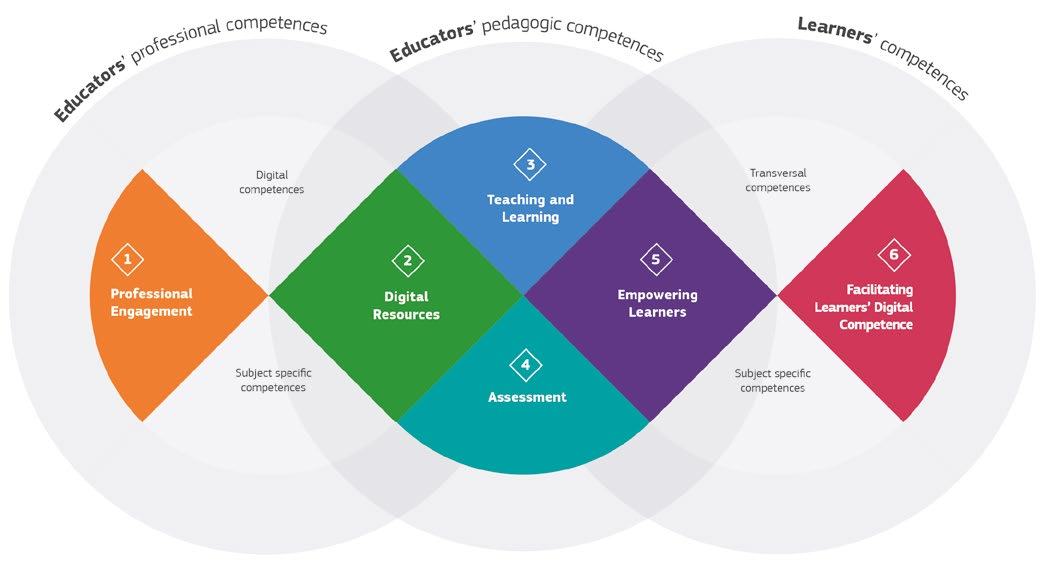
\includegraphics[width=0.9\textwidth]{fig01.png}
    \caption{Áreas y alcance del DigCompEdu.}
    \label{fig01}
    \source{\cite[p.~15]{christine_redecker_european_2017}.}
\end{figure}

%El DigCompEdu agrupa 22 competencias en 6 grandes áreas, que serían (REDECKER, 2020):
El DigCompEdu agrupa 22 competencias en 6 grandes áreas, que se presentan en la \Cref{tab02} \cite{christine_redecker_european_2017}.

\begin{table}[htbp]
    \centering
    \begin{threeparttable}
    \caption{Descriptores de las áreas DigCompEdu.}
    \label{tab02}
    \begin{tabular}{p{0.2\textwidth}p{0.7\textwidth}}
    \toprule
    Área & Descripción \\
    \midrule
    Compromiso profesional & 
    Enfocada en el entorno profesional, se materializa en la capacidad para hacer uso de tecnologías digitales para la mejora de la enseñanza y las interacciones profesionales con la comunidad educativa, para su desarrollo profesional y el bien colectivo, la innovación en la organización y la docencia. \\
    Contenidos digitales & 
    Referida a las fuentes, creación y distribución de recursos digitales, y asumiendo que el profesorado tiene acceso a multitud de recursos educativos digitales, se hace necesario que sepan identificar los recursos que respondan a los objetivos de aprendizaje planteados, a su grupo de alumnos/as, estilo de enseñanza, etc. Además de ser capaz de desarrollar sus propios recursos digitales, siendo conscientes de cómo usar y gestionar responsablemente dicho contenido digital, respetando los derechos de autor y sabiendo cómo compartirlo en red. \\
    Enseñanza y aprendizaje & 
    Centrada en cómo administrar y dirigir el uso de herramientas digitales en la enseñanza y el aprendizaje, aceptando que posibilitan la mejora de ciertas estrategias, hace alusión a su integración para el diseño, planificación e implementación de tecnologías digitales en el proceso de enseñanza - aprendizaje. \\
    Evaluación y retroalimentación &
    Alusiva a herramientas y estrategias digitales que permitan mejorar la evaluación, desde el punto de vista evaluativo, de aprendizaje y administrativo, donde es necesario que el profesorado valore de la forma de facilitar enfoques innovadores, sepa tomar decisiones en base a los datos interpretados y adapte sus estrategias según los resultados. \\
    Empoderar a los estudiantes & 
    Referida al uso de herramientas digitales para empoderar a los estudiantes, reconociendo su potencial para el apoyo de las estrategias centradas en el alumno, su participación en el proceso de enseñanza – aprendizaje y personalización. A su vez la identificación de los riesgos en el aumento de las desigualdades. \\
    Facilitar la competencia digital a los estudiantes &
    Trata sobre cómo facilitar la competencia digital de los estudiantes, desde un enfoque transversal e integral. \\
    \bottomrule
    \end{tabular}
    \source{Elaboración propia.}
    \end{threeparttable}
\end{table}

En el centro del marco de referencia, por ser el núcleo pedagógico, se sitúan las áreas de contenidos digitales, enseñanza y aprendizaje, evaluación y retroalimentación, y empoderamiento de los estudiantes, en las que se establecen las competencias que el profesorado debe dominar para incentivar estrategias de aprendizaje efectivas, inclusivas e innovadoras, empleando herramientas digitales (\Cref{fig02}).

\begin{figure}[h!]
    \centering
    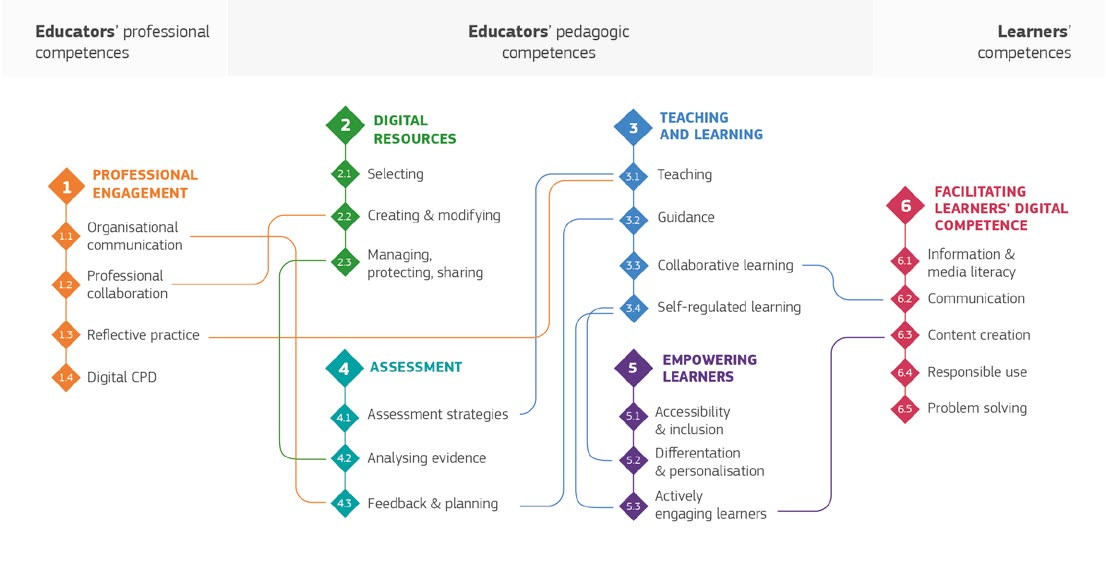
\includegraphics[width=0.9\textwidth]{fig02.png}
    \caption{Conexiones entre las competencias DigCompEdu.}
    \label{fig02}
    \source{\cite[p.~16]{christine_redecker_european_2017}.}
\end{figure}

Resaltar la dimensión “empoderamiento de los estudiantes” del Marco Europeo para la Competencia Digital Docente “DigCompEdu” \cite{christine_redecker_european_2017}, donde se inserta la participación activa del estudiantado que se traduce como la utilización de herramientas digitales para el compromiso activo, empleo de tecnologías digitales para la expresión creativa, participación activa, resolución de problemas, etc.

Pero ¿qué pasa en el ámbito social? El mundo interconectado trajo consigo distintas maneras de entender la participación en donde la modalidad de interacción en línea y en ámbitos digitales se rige, entre otras, por una transformación en el ámbito de la participación juvenil donde puedan ser protagonistas activos en las áreas de su interés.

De acuerdo con \textcite{aparici_cultura_2013} en estos ámbitos la cultura de la participación es aquella que no tiene barreras para la expresión ciudadana, que apoya la creatividad y la puesta en común de creaciones propias y colectivas. Este tipo de colaboración pasa por establecer nuevas lógicas comunicativas que abandonen la división entre emisores y receptores \cite{aparici_comunicar_2018}, para profundizar en un nuevo modelo abrazado por un ecosistema digital donde se proyectan estrategias que permitan el empoderamiento de la juventud en el plano de la comunicación.

Así, es posible ver que la influencia de las tecnologías digitales en la sociedad está promoviendo nuevos canales de comunicación nodal, especialmente entre la juventud, donde la participación se ha convertido en una interacción entre individuos que comparten ideas y tienen la capacidad de influir en el otro sobre todo cuando hablamos de integración en entornos virtuales y redes sociales \cite{torres-diaz_integracion_2013,gonzalez-lizarraga_cyberactivism:_2016,sabulsky_analiticas_2019,hernandez-selles_herramientas_2021}. Pero ¿esto se traslada a un entorno educativo formal? Esta pregunta es latente en el momento presente siendo un reto dirigido hacia la educación formal, donde el modelo de educación a distancia se ha redefinido como urgente a lo que en investigaciones previas \cite{charles_hodges_difference_2020,martinez_perez_educacion_2020,sangra_decalogo_2020,garcia_aretio_covid-19_2020} han llamado “enseñanza remota de emergencia” en época de pandemia. Pero esto no es algo que surge por efecto de la pandemia. \textcite{unesco_marco_2019} ya anunciaba este predominio de la participación de los jóvenes que los lleva a involucrarse en entornos informales de aprendizaje haciendo notar la urgencia de equiparar esta misma participación en entornos formales.

El mero hecho de un acceso a medios digitales en un contexto educativo no supone generar unos espacios alentados por una participación del alumnado, un incentivo hacia la interconexión y establecimiento de relaciones con objeto de profundizar en su aprendizaje, al menos en los contextos educativos más formales, puesto que en los diversos espacios alternativos son capaces de mantener estrechos vínculos con sus iguales desde un clima marcado por la motivación, la inquietud y los estímulos. Entonces, ¿qué elementos se muestran necesarios para trasladar este contexto a la educación superior?

La participación estudiantil depende de algunos factores tales como la estrategia pedagógica empleada por el profesorado, el ambiente que se genere en la comunidad de aprendizaje, así como las propias motivaciones del estudiantado en su propio proceso de aprendizaje. En entornos virtuales, las herramientas tecnológicas son un elemento mediador en el proceso de enseñanza y aprendizaje, y de la interacción propia de quienes forman parte de él.

\section{Espacios de Participación Invisibles. Síndrome de la Cámara Apagada}\label{sec-espacios}

Estudios sobre el uso de la cámara por videoconferencia para la enseñanza de idiomas en entornos en línea señalan la relevancia de la interacción usando dicha herramienta para lograr una presencia social e interacción \cite{codreanu_effects_2013,megha_tollefson_study_2016,delaus_influence_2016}, así como la comunicación oral y gestual de quienes interactúan como elemento primordial para generar que se involucren en los momentos en los que se interactúa en este medio \cite{satar_multimodal_2013}.

\textcite{charles_koeber_outside_2008}, en una investigación donde analizan la interacción de docentes con estudiantes universitarios en la enseñanza de contenidos sociológicos, enfatizan algunas limitantes en la comunicación significativa tanto de docentes como de estudiantes en sesiones efectuadas por videoconferencia, ya que los movimientos y gestos que presencialmente un docente hace no se equiparan a los que puede realizar frente a una cámara: los movimientos se reducen a un espacio delimitado. A su vez, otra dificultad que señalan es la falta de recepción de distintos mensajes auditivos y visuales entre quienes interactúan, lo cual lleva a no poder detectar esas señales sutiles en los comportamientos del alumnado, que conducen al docente a no poder tomar decisiones y actuar al respecto. Así, los gestos que se pueden percibir a través de la videoconferencia se tornan insignificantes para quienes interactúan por ese medio, traduciéndose en una reducción de la participación del estudiantado.

Por su parte, \textcite{martin_examining_2012} en su estudio sobre clases virtuales sincrónicas subrayan la relevancia del estilo docente y su presencia visual como factores claves para promover la interacción del estudiantado, lo cual resulta crucial para garantizar la satisfacción y la participación de estos últimos en los cursos en línea. Destacan las ventajas de las sesiones sincrónicas para promover dicha interacción sacando provecho de las funcionalidades de las plataformas que se utilicen para las videoconferencias, lo cual abre una gama de posibilidades de participación por parte del alumnado. Esto se logra siempre y cuando se potencien cuatro tipos de interacciones: estudiante-estudiante, estudiante-instructor, estudiante-contenido, estudiante-interface.

En la mayoría de los casos, se percibe el uso de la videoconferencia en sesiones sincrónicas como un elemento que permite la cercanía, la interacción en tiempo real entre estudiantes y profesorado, así como la recepción de retroalimentación inmediata para el alumnado \cite{delaus_influence_2016}.

En el contexto actual, y extendiendo el uso de la videoconferencia o videollamada más allá del entorno educativo, la situación provocada por la pandemia de la COVID-19 ha originado un empuje muy considerable al emplearse como principal medio de acercamiento entre familiares y amistades. Así, se han tratado de representar encuentros virtuales que se asemejan, lo más posible, a situaciones cotidianas vividas antes de la aparición del virus. Se ha forjado un escenario virtual donde tanto el audio como la imagen cobran especial relevancia en la participación de los interactuantes, logrando un clima marcado por la cercanía, el afecto y la sensación de un contacto más estrecho.

De acuerdo con los datos facilitados por Vodafone\footnote{Recuperado de: \url{https://cutt.ly/Flepnkq}}, por ejemplo, en España el uso de Zoom y de Hangouts aumentó en más de un 4.000 y un 2.500\% respectivamente durante los primeros meses de confinamiento (marzo y abril de 2020), mientras que Skype y las videollamadas de WhatsApp se multiplicaron por 8 y por 4 respectivamente.

La obligada transición entre un modelo educativo presencial hacia uno a distancia ha traído consigo una adopción de medidas aceleradas e irreflexivas que han dictaminado, en algunas ocasiones, un devenir problemático de los acontecimientos. En este cambio de escenario educativo no siempre es asumido la adopción de competencias y saberes digitales por parte del profesorado y alumnado que promulguen con un proceso de enseñanza aprendizaje activo y participativo, sino que existen importantes desavenencias que se han manifestado durante meses, alarmando y poniendo en relieve una necesidad imperiosa de implementar nuevas medidas de participación e interacción entre los distintos agentes que componen el acto educativo.

Este escenario descrito durante la pandemia ha evidenciado una serie de hechos como: falta de una mayor formación del profesorado sobre tecnología educativa, requerir una mejora en el nivel de competencias digitales y necesidad de un incremento en habilidades para evaluar situaciones educativas \cite{area_tecnologias_2021}.

La representación virtual del aula, en algunas ocasiones muy dispar a la de un modelo tradicional, deja vacías actuaciones cotidianas que no se equiparan de manera homogénea con su análoga, donde la interacción presencial entra en disputa con recursos digitales tales como la activación de la cámara web como herramienta en la educación superior a distancia, la cual no acaba de cobrar el protagonismo alcanzado en entornos informales, donde en ciertas ocasiones influye directamente en la calidad de la interacción \cite{brodie_consumer_2013,goldman_balancing_2011}, que resulta perjudicada.

La ausencia de un modelo estandarizado de conexión y participación en materia educativa a distancia refleja una inclinación hacia la desconexión de elementos como la cámara web o el micrófono por parte del estudiantado, dando lugar a lo que se ha denominado “síndrome de la cámara apagada”. Este fenómeno se ha tornado problemático para el profesorado ya que pierden la interacción y el contacto con el alumnado, que partiendo de un modelo e-learning precisa de la mayor contribución de elementos que hagan posible la creación de un ecosistema accesible, participativo y enriquecedor.

Una reconfiguración de la enseñanza a distancia debe pasar por el hecho de incrementar las oportunidades que se generan desde una esfera digital por parte del alumnado para fomentar su empoderamiento y capacidad de creación de contenido, pero amparados por el uso óptimo de aquellas herramientas a su alcance con objeto de brindar oportunidades de aprendizaje propias del siglo XXI. Eso que se convierte en una participación invisible se ha tornado a interpretarse como un elemento que entorpece el acontecer diario en estos procesos de enseñanza y que limita las actuaciones propias de los agentes involucrados en las mismas. Desde una perspectiva social, humanística y pedagógica se deben integrar medidas que favorezcan la activación de recursos tales como la cámara web y el micrófono, pero no desde un sentimiento amparado en la obligación, sino como una apuesta por adaptar el modelo educativo hacia un nuevo sistema donde se priorice la visibilidad del estudiantado como un sinónimo de acción, de relación y empatía.



\section{Objeto de estudio}\label{sec-objeto}
El estudio que se presenta responde a los siguientes objetivos:
\begin{itemize}
    \item Determinar el nivel del uso de la cámara en las sesiones de clase por parte del estudiantado y la percepción del mismo respecto a la competencia digital docente, metodología y prácticas docentes implementadas en clase.
    \item Determinar la metodología y la práctica docente utilizadas en clase a partir de la influencia de variables personales y contextuales.
    \item Establecer la estructura de los indicadores de metodología y práctica docente, incluyendo los factores personales y contextuales en dicha estructura.
\end{itemize}



\section{Método}\label{sec-metodo}
\subsection{Diseño de investigación}\label{sec-diseno}

El diseño de investigación es correlacional y de tipo reduccional, pues se establecen relaciones entre distintas variables y su reducción dimensional. Se trata de un estudio transversal, pues los datos se han recogido en una única administración.

\subsection{Participantes}\label{sec-participantes}

La muestra está compuesta por 142 estudiantes universitarios pertenecientes a la Universidad Internacional de Valencia (VIU). El tipo de muestreo fue por conveniencia.

Respecto a las características de la muestra, el 34.5~\% son hombres y el 65.5~\% son mujeres. Con una edad promedio en el intervalo de 30 a 35 años, y que se encuentran cursando estudios de Grado (35.9~\%) o Máster (64.1~\%) en diversas disciplinas entre las que destacan el Máster en TIC aplicadas a la Educación (44 estudiantes), Grado en Administración y Dirección de Empresas y Grado en Traducción e Interpretación (ambos con 14 estudiantes representados en la muestra) o Grado en Derecho (13 estudiantes). Mayoritariamente los encuestados residen en España (72.5~\%), aunque también nos encontramos con alumnado de Colombia (9,2~\%), México (8.5~\%) o Ecuador (2.8~\%), entre otros.

La totalidad de los participantes, presentan un nivel similar en el uso de los recursos tecnológicos, ya que están cursando sus estudios en la misma Universidad y su modelo pedagógico se basa principalmente en dos ejes: la implementación de las metodologías docentes activas y la incorporación de las TIC en el proceso de enseñanza-aprendizaje. En el caso del estudiantado que está cursando el Máster en TIC aplicadas a la Educación, se les exige unos conocimientos previos en el perfil de ingreso a dichos estudios de postgrado, para poder cursar dicha titulación.

\subsection{Instrumento}\label{sec-instrumento}
Para este estudio se ha utilizado un instrumento de recogida de información caracterizado por un cuestionario enfocado en varias dimensiones: 1) Competencia Digital del docente, donde se le solicitaba al alumnado que evaluará la competencia digital del profesorado y cuya valoración se efectúa mediante una escala tipo Likert con 5 opciones de respuesta (“nada competente” hasta “muy competente”). 2) Respecto a la percepción de la metodología docente utilizada en las sesiones por parte del estudiantado, donde se le preguntaba al alumnado sobre las metodologías activas que se implementan en las diferentes sesiones de videoconferencia de las asignaturas cursadas (7 ítems) y cuya valoración se realiza mediante una escala de Likert con 5 respuestas (desde “nunca” hasta “siempre”). Aclarar que dentro de la guía docente de todas las asignaturas de Grado y Máster, se explicita y recoge un resumen explicativo de las principales metodologías docentes que se aplicarán como parte del modelo educativo institucional y que se contemplan como estudio en esta investigación. 3) En relación con la dimensión prácticas docentes empleadas durante las sesiones de videoconferencia, se recogen los datos sobre las prácticas docentes realizadas por parte del profesorado en las sesiones de videoconferencia percibidas por el estudiantado (4 ítems) y cuya valoración se realiza mediante una escala de Likert con 5 respuestas (desde “nunca” hasta “siempre”). Igualmente, estas prácticas docentes vienen en parte sustentadas por el propio modelo educativo institucional y además por la libertad de cátedra de cada docente.

Respecto a las variables personales y contextuales se han utilizado las siguientes: país de residencia (España/Latinoamérica) y la utilización de la cámara y el micrófono, realizando dos agrupamientos (alto y bajo) en función del grado de frecuencia tanto para asuntos personales como en el ámbito académico.

\subsection{Procedimiento}\label{sec-procedimiento}
El cuestionario diseñado con Google Forms fue suministrado a través de una invitación a un universo de muestra de alumnado al que tuvimos acceso durante el curso académico 2019-2020.

Este estudio respetó las normas éticas requeridas en toda investigación, ya que al alumnado se le facilitaba el enlace del cuestionario en la plataforma utilizada, garantizando la confidencialidad, la protección de datos personales, el derecho a la información y en el que se debía marcar la casilla de consentimiento informado.

La información obtenida se tratará de acuerdo con el Reglamento General de Protección de Datos, así como a la Ley Orgánica 3/2018, de 5 de diciembre, de Protección de Datos Personales y Garantía de los Derechos Digitales. El alumnado que respondió a las cuestiones planteadas en dicho instrumento, se entiende, de forma tácita, que ha comprendido los objetivos del presente estudio y que acepta participar en esta investigación.

\subsection{Análisis}\label{sec-analisis}

Los datos han sido analizados a través del programa SPSS 24 (con la Licencia de la Universidad Internacional de Valencia). Se ha realizado estadísticos descriptivos de las dimensiones contempladas, Análisis Multivariado de Varianza (MANOVA) y Análisis de Varianza (ANOVA), y por último se ha utilizado el análisis de Componentes Principales Categórico (CATPCA) para sintetizar la información obtenida.

\subsection{Resultados}\label{sec-resultados}

En primer lugar, se presentan los estadísticos descriptivos de los tres apartados contemplados: competencia digital docente, metodología y prácticas docentes. Seguidamente, se muestra la influencia de los factores personales y contextuales respecto a la metodología y prácticas docentes. Finalmente, se determina la estructura de las dos dimensiones y las variables de influencia.

\subsubsection{Nivel de Competencia Digital Docente, Metodología y Prácticas Docente}
La competencia digital docente valorada por el estudiantado presenta un nivel promedio alto. En relación con la metodología docente, la clase magistral sigue siendo la más utilizada, seguida por el trabajo colaborativo, el trabajo autónomo y el estudio de casos, como se puede apreciar en la \Cref{tab03}. Las metodologías menos empleadas son las basadas en las tutorías y en las simulaciones, situándose por debajo del 3 en la escala.  En todos los indicadores que se analizan se aprecia una variabilidad alta, con lo cual las respuestas del alumnado son heterogéneas.

\begin{table}[h]
    \centering
    \begin{threeparttable}
    \caption{Descriptivos de los apartados competencia digital, metodología y prácticas docentes.}
    \label{tab03}
    \begin{tabular}{p{0.6\textwidth}cc}
    \toprule
    Nivel de Competencia Docente & Media & Desviación típica \\
    \midrule
    Valoración del Nivel de Competencia Docente por parte del estudiantado & 4.06 & 0.83 \\
    \midrule
    Metodología Docente & & \\
    \midrule
    Clase Magistral & 3.96 & 0.92 \\
    Estudio de Casos & 3.01 & 1.05 \\
    Learning by Doing & 3.16 & 1.13 \\
    Trabajo Colaborativo & 3.38 & 1.02 \\
    Tutorías & 2.76 & 1.26 \\
    Simulación & 2.12 & 1.10 \\
    Trabajo Autónomo & 3.12 & 1.03 \\
    Total & 3.96 & 0.92 \\
    \midrule
    Prácticas Docentes & & \\
    \midrule
    Recursos & 4.13 & 0.99 \\
    Espacios y Participación & 3.90 & 1.02 \\
    Contenido & 4.30 & 0.92 \\
    Trabajo Colaborativo & 3.59 & 1.19 \\
    Total & 4.13 & 0.99 \\
    \bottomrule
    \end{tabular}
    \source{Elaboración propia.}
    \end{threeparttable}
\end{table}


\subsubsection{Influencia en las variables personales y contextuales en la metodología y prácticas docentes}

En este apartado se analiza y se plasman las diferencias en la metodología docente y las prácticas docentes a partir de la variable país de residencia, utilización de la cámara y competencia digital docente. Para ello, se han llevado a cabo análisis MANOVA y ANOVA.

\subsubsection{País}

En relación con la metodología y la práctica docente en función del país de residencia, las medias entre el alumnado de España y el alumnado de Latinoamérica son diferentes entre sí (\Cref{tab04}. Los valores medios más altos en ambos casos se sitúan en la metodología de clase magistral y el trabajo colaborativo, y en las prácticas docentes relacionadas con el contenido y los recursos. Los valores más bajos se sitúan en ambos casos en la metodología basada en la simulación.  

En relación con la metodología, en todos los casos, exceptuando la clase magistral y el estudio de casos, el alumnado de Latinoamérica presenta promedios superiores al valorar el uso de las metodologías activas por parte del profesorado. Sin embargo, respecto a las prácticas docentes, se presentan valores promedios similares entre el alumnado de ambos países.  

Las diferencias encontradas, a nivel multivariado son estadísticamente significativas (Lambda de Wilks$=.724$; $F(11, 130)=4.505$; $p=.000$), con un tamaño del efecto grande ($\eta^2$ parcial $=.276$). Desde el análisis univariado (ANOVA), -ver \Cref{tab03}-, casi todos los indicadores de metodología son estadísticamente significativos, a excepción del estudio de casos y la simulación. La metodología de clase magistral, trabajo colaborativo y el trabajo autónomo presentan un tamaño del efecto pequeño, mientras que en la metodología Learning by doing y tutorías es grande. Respecto a las prácticas docentes, no se producen diferencias significativas en ningún indicador contemplado.  


\begin{table}[h]
    \centering
    \begin{threeparttable}
    \caption{Descriptivos en función del país de Residencia y ANOVA en los apartados de metodología y práctica docente.}
    \label{tab04}
    \begin{tabular}{*{7}{l}}
    \toprule
    Metodología Docente & Grupo & Media & Desv. típica & F & Sig. & $\eta^2$ parcial \\
    \midrule
    \multirow{2}{*}{MT\_Clase Magistral} & ES & 4.09 & 0.86 & \multirow{2}{*}{6.850} & \multirow{2}{*}{.010} & \multirow{2}{*}{.010} \\
    & LATAM & 3.64 & 1.01 & & & \\
    \multirow{2}{*}{MT\_Estudio de Casos} & ES & 3.05 & 1.02 & \multirow{2}{*}{.578} & \multirow{2}{*}{.448} & \multirow{2}{*}{.004} \\
    & LATAM & 2.90 & 1.14 & & & \\
    \multirow{2}{*}{MT\_Learning by Doing} & ES & 3.05 & 1.08 & \multirow{2}{*}{9.772} &  \multirow{2}{*}{.002} & \multirow{2}{*}{.108} \\
    & LATAM & 3.46 & 1.21 & & & \\
    \multirow{2}{*}{MT\_Trabajo Colaborativo} & ES & 3.30 & 0.98 & \multirow{2}{*}{3.828} & \multirow{2}{*}{.050} & \multirow{2}{*}{.027} \\
    & LATAM & 3.59 & 1.04 & & & \\
    \multirow{2}{*}{MT\_Tutorías} & ES & 2.50 & 1.21 & \multirow{2}{*}{18.545} & \multirow{2}{*}{.000} & \multirow{2}{*}{.117} \\
    & LATAM & 3.46 & 1.14 & & & \\
    \multirow{2}{*}{MT\_Simulación} & ES & 2.03 & 1.05 & \multirow{2}{*}{2.536} & \multirow{2}{*}{.114} & \multirow{2}{*}{.018} \\
    & LATAM & 2.36 & 1.22 & & & \\
    \multirow{2}{*}{MT\_Trabajo Autónomo} & ES & 2.94 & 1.34 & \multirow{2}{*}{6.676} & \multirow{2}{*}{.011} & \multirow{2}{*}{.046} \\
    & LATAM & 3.59 & 1.29 & & & \\
%    \multirow{2}{*}{} & & & & \multirow{2}{*}{} & \multirow{2}{*}{} & \multirow{2}{*}{} \\
%    &  & & & \\
    \midrule
    Prácticas Docentes & & & & & & \\
    \midrule
    \multirow{2}{*}{PD\_Recursos} & ES & 4.20 & 1.01 & \multirow{2}{*}{1.860} & \multirow{2}{*}{.175} & \multirow{2}{*}{.013} \\
    & LATAM & 3.95 & 0.94 & & & \\
    \multirow{2}{*}{PD\_Participación} & ES & 3.83 & 1.03 & \multirow{2}{*}{1.622} & \multirow{2}{*}{.205} & \multirow{2}{*}{.011} \\
    & LATAM & 4.08 & 0.92 & & & \\
    \multirow{2}{*}{PD\_Contenido} & ES & 4.38 & 0.84 & \multirow{2}{*}{2.562} & \multirow{2}{*}{.112} & \multirow{2}{*}{.018} \\
    & LATAM & 4.10 & 1.09 & & & \\
    \multirow{2}{*}{PD\_Trabajo Colaborativo} & ES & 3.61 & 1.14 & \multirow{2}{*}{.106} & \multirow{2}{*}{.745} & \multirow{2}{*}{.001} \\
    & LATAM & 3.54 & 1.31 & & & \\
    \bottomrule
    \end{tabular}
    \source{Elaboración propia.}
    \end{threeparttable}
\end{table}


\subsection{Utilización de la cámara en las sesiones}
En este apartado, a partir de la utilización de la cámara en las sesiones se han constituido dos grupos: bajo y alto. El grupo alto está formado por el alumnado que utiliza asiduamente la cámara en las sesiones sincrónicas, mientras que el grupo bajo lo compone el alumnado que no utiliza la cámara en las sesiones de videoconferencia y los principales motivos que argumentan son los siguientes: 1) Privacidad, ya que el entorno virtual no permite establecer fondo. 2) Porque no es obligatorio y 3) Por vergüenza e inseguridad. Ahora bien, en grupos reducidos, el conjunto del alumnado se muestra más proclive para encender la cámara.

El conjunto del alumnado que no utiliza la cámara en las videoconferencias valora sus sesiones como clases magistrales, mientras que el grupo de alumnado que participa con la cámara encendida argumenta que en las sesiones se utiliza otro tipo de metodologías docentes más activas. Sucede lo mismo con la dimensión de prácticas docentes.

Los valores medios más altos se sitúan en la metodología de clase magistral y el trabajo colaborativo, así como en las prácticas docentes basadas en la transmisión de contenidos y la facilitación de recursos por parte del docente.  

Las diferencias encontradas, a nivel multivariado, son estadísticamente significativas (Lambda de Wilks $=.698$; $F(11, 130)=5.119$; $p=.000$), con un tamaño del efecto grande ($\eta^2$ parcial $=.302$). Desde el análisis univariado (ANOVA) (\Cref{tab05}), casi todos los indicadores de metodología son estadísticamente significativos, a excepción de la metodología de clase magistral. El trabajo colaborativo y el trabajo autónomo presentan un tamaño del efecto pequeño, el estudio de casos y la metodología learning by doing es mediano y, por último, las tutorías y la metodología basada en la simulación el tamaño del efecto es grande. Respecto a los indicadores que hacen referencia a las prácticas docentes, ninguno de ellos es estadísticamente significativo.

\begin{table}[h]
    \centering
    \begin{threeparttable}
    \caption{Descriptivos en función la utilización de la cámara en las sesiones y ANOVA en los apartados de metodología y práctica docente.}
    \label{tab05}
    \begin{tabular}{*{7}{l}}
    \toprule
    Metodología Docente & Grupo & Media & Desv. típica & F & Sig. & $\eta^2$ parcial \\
    \midrule
    \multirow{2}{*}{MT\_Clase Magistral} & Bajo & 4.04 & 0.85 & \multirow{2}{*}{2.488} & \multirow{2}{*}{.117} & \multirow{2}{*}{.017} \\
    & Alto & 3.76 & 1.07 & & & \\
    \multirow{2}{*}{MT\_Estudio de Casos} & Bajo & 2.82 & 1.00 & \multirow{2}{*}{13.697} & \multirow{2}{*}{.000} & \multirow{2}{*}{.089} \\
    & Alto & 3.53 & 1.00 & & & \\
    \multirow{2}{*}{MT\_Learning by Doing} & Bajo & 2.96 & 1.11 & \multirow{2}{*}{13.194} &  \multirow{2}{*}{.000} & \multirow{2}{*}{.086} \\
    & Alto & 3.71 & 1.01 & & & \\
    \multirow{2}{*}{MT\_Trabajo Colaborativo} & Bajo & 3.28 & 1.00 & \multirow{2}{*}{4.014} & \multirow{2}{*}{.047} & \multirow{2}{*}{.028} \\
    & Alto & 3.66 & 0.94 & & & \\
    \multirow{2}{*}{MT\_Tutorías} & Bajo & 2.41 & 1.10 & \multirow{2}{*}{36.613} & \multirow{2}{*}{.000} & \multirow{2}{*}{.207} \\
    & Alto & 3.61 & 0.92 & & & \\
    \multirow{2}{*}{MT\_Simulación} & Bajo & 1.86 & 0.94 & \multirow{2}{*}{25.983} & \multirow{2}{*}{.015} & \multirow{2}{*}{.157} \\
    & Alto & 2.84 & 1.19 & & & \\
    \multirow{2}{*}{MT\_Trabajo Autónomo} & Bajo & 2.94 & 1.37 & \multirow{2}{*}{6.885} & \multirow{2}{*}{.010} & \multirow{2}{*}{.047} \\
    & Alto & 3.61 & 1.19 & & & \\
    \midrule
    Prácticas Docentes & & & & & & \\
    \midrule
    \multirow{2}{*}{PD\_Recursos} & Bajo & 3.97 & 0.91 & \multirow{2}{*}{1.339} & \multirow{2}{*}{.249} & \multirow{2}{*}{.009} \\
    & Alto & 4.10 & 1.02 & & & \\
    \multirow{2}{*}{PD\_Participación} & Bajo & 3.86 & 0.99 & \multirow{2}{*}{.788} & \multirow{2}{*}{.376} & \multirow{2}{*}{.006} \\
    & Alto & 4.03 & 1.37 & & & \\
    \multirow{2}{*}{PD\_Contenido} & Bajo & 4.37 & 0.88 & \multirow{2}{*}{1.798} & \multirow{2}{*}{.182} & \multirow{2}{*}{.013} \\
    & Alto & 4.13 & 1.08 & & & \\
    \multirow{2}{*}{PD\_Trabajo Colaborativo} & Bajo & 3.58 & 1.20 & \multirow{2}{*}{.006} & \multirow{2}{*}{.940} & \multirow{2}{*}{.000} \\
    & Alto & 3.60 & 1.05 & & & \\
    \bottomrule
    \end{tabular}
    \source{Elaboración propia.}
    \end{threeparttable}
\end{table}



\subsubsection{Competencia Digital Docente}
En este apartado, a partir de la competencia digital docente percibida por el alumnado se han constituido dos grupos: bajo y alto. El conjunto de profesores -valorado por el alumnado- que presenta un nivel de competencia alto, según el alumnado utiliza metodologías más activas e innovadoras, mientras que el profesorado que pertenece al grupo bajo se inclina por el uso de aquellas de corte más magistral y pasivo.  

Las diferencias encontradas, a nivel multivariado son estadísticamente significativas (Lambda de Wilks $=.763$; $F(11, 130)=3.667$; $p=.000$), con un tamaño del efecto grande ($\eta^2$ parcial $=.237$). Desde el análisis univariado (ANOVA) (\Cref{tab06}), casi todos los indicadores referentes a la metodología son estadísticamente significativos con un tamaño del efecto mediano, a excepción de la metodología de clase magistral que no es estadísticamente significativa, como en los casos anteriores. Las principales diferencias entre ambos grupos se producen en las tutorías learning by doing y el estudio de casos, por tanto, a mayor competencia digital docente mayor implementación de metodologías activas en el aula. Respecto a los indicadores de prácticas docentes, casi todos los indicadores son estadísticamente significativos con un tamaño del efecto pequeño, a excepción de la práctica docente basada en la participación.

\begin{table}[h]
    \centering
    \begin{threeparttable}
    \caption{Descriptivos en función de la Competencia Digital Docente y ANOVA en los apartados de metodología y práctica docente.}
    \label{tab06}
    \begin{tabular}{*{7}{l}}
    \toprule
    Metodología Docente & Grupo & Media & Desv. típica & F & Sig. & $\eta^2$ parcial \\
    \midrule
    \multirow{2}{*}{MT\_Clase Magistral} & Bajo & 4.09 & 0.92 & \multirow{2}{*}{1.855} & \multirow{2}{*}{.278} & \multirow{2}{*}{.008} \\
    & Alto & 3.91 &0.92 & & & \\
    \multirow{2}{*}{MT\_Estudio de Casos} & Bajo & 2.78 & 0.96 & \multirow{2}{*}{16.950} & \multirow{2}{*}{.000} & \multirow{2}{*}{.108} \\
    & Alto & 3.52 & 1.06 & & & \\
    \multirow{2}{*}{MT\_Learning by Doing} & Bajo & 2.90 & 1.05 & \multirow{2}{*}{19.382} &  \multirow{2}{*}{.000} & \multirow{2}{*}{.122} \\
    & Alto & 3.75 & 1.10 & & & \\
    \multirow{2}{*}{MT\_Trabajo Colaborativo} & Bajo & 3.17 & 0.92 & \multirow{2}{*}{14.575} & \multirow{2}{*}{.000} & \multirow{2}{*}{.094} \\
    & Alto & 3.84 & 1.05 & & & \\
    \multirow{2}{*}{MT\_Tutorías} & Bajo & 2.45 & 1.18 & \multirow{2}{*}{20.401} & \multirow{2}{*}{.000} & \multirow{2}{*}{.127} \\
    & Alto & 3.43 & 1.18 & & & \\
    \multirow{2}{*}{MT\_Simulación} & Bajo & 1.97 & 1.02 & \multirow{2}{*}{6.035} & \multirow{2}{*}{.015} & \multirow{2}{*}{.041} \\
    & Alto & 2.45 & 1.22 & & & \\
    \multirow{2}{*}{MT\_Trabajo Autónomo} & Bajo & 2.94 & 1.32 & \multirow{2}{*}{5.785} & \multirow{2}{*}{.017} & \multirow{2}{*}{.040} \\
    & Alto & 3.52 & 1.37 & & & \\
    \midrule
    Prácticas Docentes & & & & & & \\
    \midrule
    \multirow{2}{*}{PD\_Recursos} & Bajo & 4.01 & 1.20 & \multirow{2}{*}{4.987} & \multirow{2}{*}{.027} & \multirow{2}{*}{.034} \\
    & Alto & 4.41 & 0.89 & & & \\
    \multirow{2}{*}{PD\_Participación} & Bajo & 3.89 & 0.99 & \multirow{2}{*}{.057} & \multirow{2}{*}{.811} & \multirow{2}{*}{.000} \\
    & Alto & 3.93 & 1.06 & & & \\
    \multirow{2}{*}{PD\_Contenido} & Bajo & 4.19 & 0.96 & \multirow{2}{*}{4.521} & \multirow{2}{*}{.035} & \multirow{2}{*}{.031} \\
    & Alto & 4.55 & 0.79 & & & \\
    \multirow{2}{*}{PD\_Trabajo Colaborativo} & Bajo & 3.42 & 1.17 & \multirow{2}{*}{6.959} & \multirow{2}{*}{.009} & \multirow{2}{*}{.047} \\
    & Alto & 3.98 & 1.19 & & & \\
    \bottomrule
    \end{tabular}
    \source{Elaboración propia.}
    \end{threeparttable}
\end{table}

\subsubsection{Estructura dimensional del uso de los recursos tecnológicos en el plano del tiempo libre y académico}

En este apartado se presenta la estructura dimensional de la metodología docente (clase magistral, estudio de casos, learning by doing, trabajo colaborativo, tutorías, simulación y trabajo autónomo) y las prácticas docentes (recursos, participación, contenido y trabajo colaborativo).

Además, se han considerado dentro de la estructura las variables personales y contextuales, como país, utilización de la cámara en las sesiones y la competencia digital docente percibida por el alumnado.  

Para ello, dado la métrica de las variables, se ha optado por realizar un análisis de componentes principales para datos categóricos (CATPCA) con el propósito de generar una estructura dimensional mediante la reducción relacional entre las variables e integrar dentro de la misma los factores personales y contextuales.

\begin{table}[h]
    \centering
    \begin{threeparttable}
    \caption{Resumen del modelo.}
    \label{tab07}
    \begin{tabular}{*{4}{l}}
    \toprule
     & & \multicolumn{2}{l}{Varianza} \\
    Dimensión & Alfa de Cronbach & Total (Autovalor) & Porcentaje \\
    \midrule
    1 & .801 & 3.681 & 33.5 \\
    2 & .529 & 1.928 & 17.5 \\
    Total & .904 & 5.610 & 51.0 \\
    \bottomrule
    \end{tabular}
    \source{Elaboración propia.}
    \end{threeparttable}
\end{table}


En función de los resultados se ha optado por un modelo de dos dimensiones de acuerdo con los valores propios encontrados –ver \Cref{tab07}- que explica el 51.0~\% de la varianza total del mismo. Además, el coeficiente α de Cronbach global ($.904$) indica que el modelo sugerido presenta un buen ajuste. La primera dimensión es considerablemente la más relevante (33.5~\% de la varianza total del modelo y un $\alpha$ de Cronbach de $.801$) erigiéndose en la dimensión principal. La segunda dimensión contribuye con menor porcentaje de varianza explicada que la primera (17.5~\% de la varianza total del modelo), si bien su valor de $\alpha$ de Cronbach ($.529$) sugiere que es una dimensión importante en la explicación del modelo.

La primera dimensión es la que más contribuye a la explicación del modelo (65.68~\% de la varianza total explicada). En ella se sitúan todos los indicadores de uso analizados en la parte positiva de la dimensión (\Cref{tab08} y \Cref{fig02}), distinguiéndose dos agrupaciones. En la primera se agrupan todos los indicadores relativos a las prácticas docentes y a la metodología de clase magistral (primer cuadrante), mientras que la segunda agrupa a todos los indicadores de la metodología docente (cuarto cuadrante).

La segunda dimensión representa una explicación media del modelo (34.31~\% de la varianza total explicada). Esta dimensión supone la diferenciación entre la metodología y la práctica docente. De esta forma, en el polo positivo de la segunda dimensión se agrupan todos los indicadores de las prácticas docentes y la metodología de clase magistral (primer cuadrante), mientras que en el polo negativo se agrupan los indicadores de metodologías docentes activas (cuarto cuadrante).

\begin{table}[h!]
    \centering
    \begin{threeparttable}
    \caption{Saturaciones.}
    \label{tab08}
    \begin{tabular}{*{3}{l}}
    \toprule
    Metodología Docente & Dimensión 1 & Dimensión 2 \\
    \midrule
    Clase Magistral & .321 & .398 \\
    Estudio de Casos & .636 & -.304 \\
    Learning by Doing & .712 & -.332 \\
    Trabajo Colaborativo & .704 & -.163 \\
    Tutorías & .628 & -.438 \\
    Simulación & .599 & -.477 \\
    Trabajo Autónomo & .482 & -.251 \\
    \midrule
    Práctica Docente & & \\
    \midrule
    Recursos & .551 & .566 \\
    Espacios y Participación & .481 & .493 \\
    Contenido & .576 & .609 \\
    Trabajo Colaborativo & .565 & .353 \\
    \bottomrule
    \end{tabular}
    \source{Elaboración propia.}
    \end{threeparttable}
\end{table}

Por lo que respecta a las variables personales y contextuales, se puede apreciar respecto al país, que el estudiantado latinoamericano percibe que en las sesiones sincrónicas se utilizan metodologías más activas que el alumnado español, como se aprecia a partir de la primera dimensión.

En referencia a la utilización de la cámara en las sesiones sincrónicas, se puede observar, desde la primera dimensión, la diferencia entre la implementación de las metodologías contempladas, siendo la metodología de clase magistral la más utilizada en ambos grupos. Sin embargo, la segunda dimensión aglutina al grupo alto en utilización de la cámara con la preferencia de la implementación de metodologías más activas y a los del grupo bajo con la metodología y prácticas docentes más pasivas.

Por último, en relación con la percepción del alumnado respecto a la competencia digital docente del profesorado, la primera dimensión diferencia claramente al grupo alto en competencia digital y al grupo bajo. A mayor nivel competencial, realizan un mayor uso de las metodologías activas -parte positiva de la dimensión- en comparación de los que poseen un nivel bajo de competencia digital -parte negativa de la dimensión-. A partir de la segunda dimensión se puede observar cómo el grupo alto de competencia digital se enfoca hacia la valoración de metodologías más activas (\Cref{fig03}).  

\begin{figure}[h!]
    \centering
    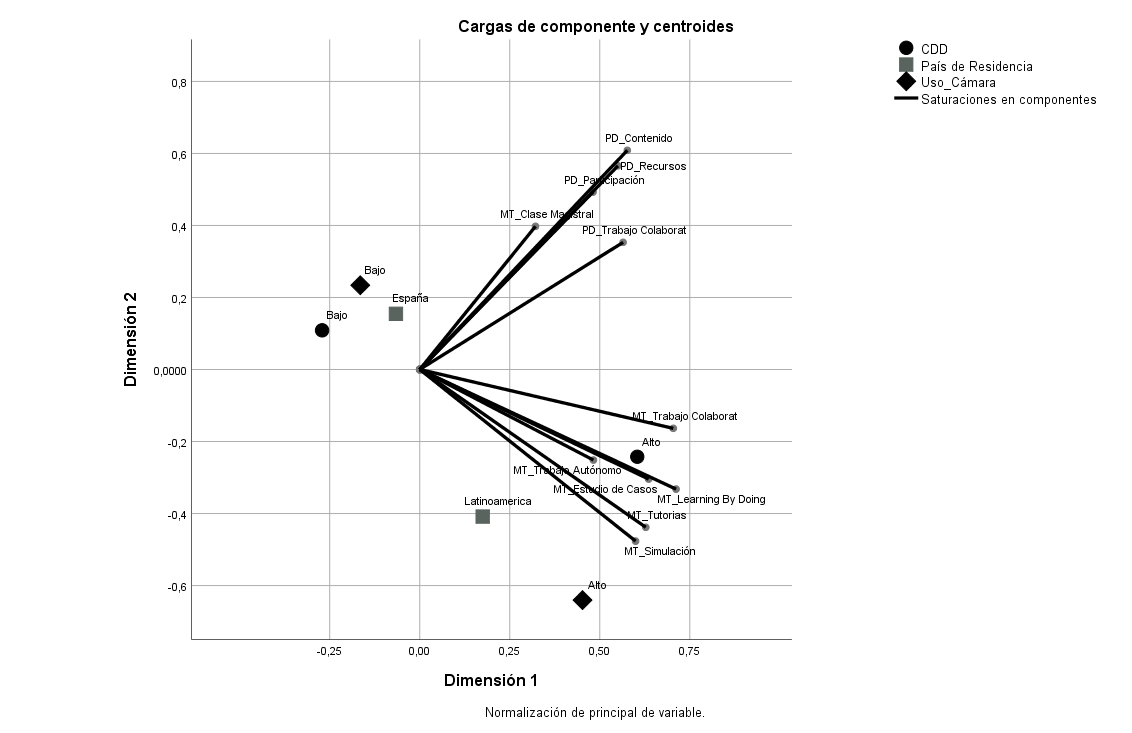
\includegraphics[width=0.9\textwidth]{fig03.png}
    \caption{Estructura dimensional de la metodología y práctica docente.}
    \label{fig03}
    \source{Elaboración propia.}
\end{figure}

\section{Conclusiones}

Los resultados de esta investigación, si bien son exploratorios, dan luz para conocer cómo se desarrollan las dinámicas de participación del estudiantado en sesiones sincrónicas por videoconferencia, y que van más allá de la propia metodología que el profesorado emplea.

La influencia de la metodología en el uso de la cámara web por parte de los estudiantes presenta una estrecha relación dado que, atendiendo a los datos de los encuestados, el uso de metodología docente basada en la clase magistral sigue siendo predominante en las clases a distancia frente a un modelo más actual y práctico como el Learning by Doing o las simulaciones; lo que promueve un rol protagonista del profesor y relega al alumnado a una actitud más pasiva que no fomenta la participación y, por ende, la activación de la cámara. Asimismo, en la práctica docente observamos cómo los contenidos siguen siendo prioritarios en el proceso de enseñanza-aprendizaje, diezmando otros recursos que involucren al estudiantado.

El alumnado que enciende la cámara de manera regular en las sesiones sincrónicas lo atribuye, en parte, al uso de pedagogías activas y participativas por parte del profesorado, mientras que aquellos estudiantes que no hacen uso de la cámara lo argumentan desde actitudes como la no obligatoriedad, la vergüenza o la inseguridad.

Se evidencia el hecho de que el alumnado que ha formado parte del estudio evalúe a sus docentes como altamente capacitados en competencia digital, estableciendo una vinculación entre el nivel competencia digital del profesorado y el uso de la cámara en videoconferencias por parte del estudiantado. En el conjunto de la muestra, tras su análisis, se refleja la relación entre la competencia digital docente y la elección de metodologías de diversa índole. Mientras que aquellos profesores que presentan un nivel más bajo de competencia digital se inclinan por metodologías centradas en la clase magistral y en la transmisión de contenidos. En cambio, los docentes valorados con un nivel de competencia digital más alto hacen uso de metodologías más activas, innovadoras y centradas en la participación activa y crítica del estudiantado en su aprendizaje, tales como Learning By Doing, estudio de casos o simulaciones.

El estudio y análisis que se ha llevado a cabo para esta esta investigación expone que a pesar de que algunos estudiantes presentan de inicio actitudes reticentes hacia el encendido de la cámara web en las sesiones sincrónicas a distancia, estas pueden cambiar potenciando el uso de metodologías activas e innovadoras y promoviendo un rol protagonista en el estudiantado, que les motive hacia una participación significativa en las clases. Asimismo, el nivel de competencia digital docente influye en la elección de una metodología más o menos activa, marcando el proceso de aprendizaje de los estudiantes e, indirectamente, el uso de la cámara web.

De ahí que sea necesario incentivar distintas vías de participación que beneficie a todo el alumnado, no solo a aquellos que enciendan sus cámaras.

En cuanto a las limitaciones que presenta el estudio es que se circunscribe al estudiantado universitario de la Universidad Internacional de Valencia, con lo que se necesitan más estudios en otras universidades, países y regiones que corroboren la temática estudiada. Además, se debe considerar que cada Universidad tiene un programa educativo o modelo pedagógico diferente que pueden incidir en los resultados obtenidos.

A la luz de estas cuestiones, y coincidiendo con \textcite{coll_aprender_2009} en no atribuir solamente a los elementos pedagógicos y didácticos el peso de los alcances de las TIC en educación ya que sería una perspectiva determinista y reduccionista del fenómeno, es relevante apreciar la práctica que se genera tanto por el alumnado como profesorado para planificar, regular y orientar las actividades propias y ajenas usando la tecnología. Y, dentro de esta práctica, la recreación y la redefinición que hacen de las actividades conjuntas en donde no solamente se da un abordaje de un contenido específico, sino que se desprende una organización, reglas implícitas o explícitas, actuaciones y significados de lo que engloba dicha práctica.

Así, un elemento relevante para futuras investigaciones sería indagar, no solo el encendido de una cámara como un equivalente a estar presente y participar en una sesión sincrónica, sino que esta participación sea realmente activa y se consiga un empoderamiento digital del alumnado.

Se hace necesario configurar un marco tecnopedagógico que dé sustento epistemológico al diseño de comunidades de aprendizaje colaborativas que contemplen los avances culturales y sociales del entorno y, sobre todo, de la vida en un mundo virtual y digital. Tal diseño deberá generar experiencias y prácticas educativas de propuestas inmersivas, placenteras, colectivas, transformadoras y originales \cite{maggio_practicas_2020}.






\printbibliography\label{sec-bib}
% if the text is not in Portuguese, it might be necessary to use the code below instead to print the correct ABNT abbreviations [s.n.], [s.l.]
%\begin{portuguese}
%\printbibliography[title={Bibliography}]
%\end{portuguese}


%full list: conceptualization,datacuration,formalanalysis,funding,investigation,methodology,projadm,resources,software,supervision,validation,visualization,writing,review
\begin{contributors}[sec-contributors]
\authorcontribution{Francisco Recio-Muñoz}[conceptualization,datacuration,investigation,projadm,supervision,writing]
\authorcontribution{Jorge Martínez-Pérez}[conceptualization,datacuration,investigation,writing]
\authorcontribution{Sara Cebrián Cifuentes}[conceptualization,datacuration,investigation,formalanalysis,methodology,writing]
\end{contributors}



\end{document}

